\documentclass[]{report}
\usepackage{geometry}
\usepackage{graphicx}
\usepackage{physics}
\usepackage{color}
\usepackage{subcaption}
\usepackage{lipsum}
\usepackage{amsmath}
\usepackage{amsfonts}
\usepackage{amssymb}
\usepackage[hidelinks]{hyperref}
\usepackage{parskip}
\usepackage{tikz}
\usetikzlibrary{shapes.callouts, shapes.geometric, arrows}
\tikzset{
	level/.style = {
		ultra thick,
		black,
	},
	connect/.style = {
		dashed,
		black
	},
	notice/.style = {
		draw,
		rectangle callout,
		callout relative pointer={#1}
	},
	label/.style = {
		text width=2cm
	}
}
\tikzstyle{arrow} = [<->,>=stealth]

\newcommand{\up}{\fbox{$\uparrow\phantom{\downarrow}$}}%
\newcommand{\dwn}{\fbox{$\phantom{\uparrow}\downarrow$}}%
\newcommand{\updwn}{\fbox{$\mathord\uparrow\downarrow$}}%
\newcommand{\emp}{\fbox{$\phantom{\downarrow}\phantom{\downarrow}$}}%
\newcommand{\electron}[2]{{%
		\setlength\tabcolsep{0pt}% remove extra horizontal space from tabular
		      %\setlength\fboxrule{0.2pt}% uncomment for original line width
		\begin{tabular}{c}
			\fboxsep=0pt\fbox{\fboxsep=3pt#2}\\[2pt]
			#1
		\end{tabular}%
}}

%\geometry{top = 2.5cm, bottom = 2.5cm, left = 2.5cm, right = 2.5cm}
%
\setlength{\parindent}{0mm}
%\setlength{\parskip}{0.5mm}

% Title Page
\title{A Study of the t-J Model\vspace{-5mm}}
\author{Amit Bikram Sanyal}
\date{Submitted on \today}

\newcommand{\I}{\,\mathrm{i}\,}

%\let\cleardoublepage=\clearpage

\begin{document}
	
\begin{minipage}{\linewidth}
	\maketitle
\end{minipage}

\vfill

\begin{center}
	\includegraphics[width=0.4\linewidth]{images/niser-logo}
\end{center}


\newpage
\tableofcontents
\thispagestyle{empty}

\begin{abstract}
	\lipsum[1]
\end{abstract}

\chapter{The Hubbard model with strong interactions}
\section{Introduction}
The Hubbard model is one of the simplest many-body models. The one-dimensional model consists of an array of $ N $ sites with $ L $ fermions. The Hubbard model captures the effect of the electrons hopping from site to site, causing the electrons to de-localize and give rise to metallic behaviour, as well the effect of strong electron-electron interactions that cause the system to go to insulating states.

The one-dimensional Hubbard Hamiltonian with nearest-neighbour hopping is given as:
\begin{align}
	\hat{H} = -t \sum_{\langle j, i \rangle } \sum_{\sigma} \left( c^{\dagger}_{j, \sigma} + c^{}_{i, \sigma} \right) + U \sum_{j} \hat{n_{i, \uparrow}} \hat{n_{j, \downarrow}}
\end{align}

where $ t $ denotes the hopping constant and $ U $ is the interaction energy cost when two fermions of opposite spins occupy the same site. The Hubbard model is a tight-binding model, in the sense that particles are localized on each site by Wannier functions and can only jump from site to site, without occupying any intermediate position.

\section{Spectrum of the interacting system}\label{sec:spectrum}
The basis of a single site labelled $ i $ the Hubbard model consists of four possible states.
\begin{enumerate}
	\item The empty site: $ \ket{0}_i $
	\item The singly occupied site with an up spin: $ \ket{\uparrow}_i = c^{\dagger}_{i, \uparrow} \ket{0}_i$ 
	\item The singly occupied site with a down spin: $ \ket{\uparrow}_i = c^{\dagger}_{i, \downarrow} \ket{0}_i$
	\item The doubly occupied site: $ \ket{\uparrow\downarrow}_i = c^{\dagger}_{i, \uparrow} c^{\dagger}_{i, \downarrow} \ket{0}_i $, denoted as $ \ket{d}_i $ this point onward.
\end{enumerate}

This convention regarding $ \ket{d}_i $ has been maintained, which means $$ c^{\dagger}_{i, \downarrow} c^{\dagger}_{i, \uparrow}  \ket{0}_i  = - c^{\dagger}_{i, \uparrow} c^{\dagger}_{i, \downarrow} \ket{0}_i = -\ket{d}_i $$.

The spectrum of the Hubbard model is parametrized by the filling ratio, $ n = N/L $ and the relative interaction strength, $ U/t $. We shall now investigate the nature of the spectrum of the Hubbard model by varying these parameters.

First, we turn off both the hopping and the interaction, that is, we set $ t=0 $ and $ U=0 $. Let the on-site energy of each site to be $ \epsilon_0$. At $ t=0 $, each single site becomes isolated, and electrons are not allowed to hop to adjacent sites. Also Each site can be empty, or singly- or doubly-occupied. But since $ U=0 $ as well, the doubly-occupied state also does not cause any change in energy to the system. This gives rise to the single, four-fold degenerate energy level at $ E=\epsilon_0 $ for all four occupation states of each electron. For $ L $ electrons in the system, the spectrum consists of $ L $ copies of the level.

Now, we turn on $ U $ to a non-zero value. The empty and the singly-occupied states are still at $ E = \epsilon_0 $, while the states with double occupation now separate into the $ E = \epsilon_0 + U $ level. The interaction, thus, lifts the degeneracy between states of each electron.

Again, let us separately consider the case of $ U = 0 $ and $ t \ne 0 $. Due to hopping, the kinetic energy term causes the spectrum to broaden into a band of width $ 2zt $,\textit{bandwidth}, where $ z $ depends on the number of particles in the system as well the effective space available to them for hopping. Therefore, hopping lifts the degeneracy between the levels of the different electrons in the system.

When both hopping and interactions are present in the system, the spectrum splits into different bands. For example, consider a system with $ L $ electrons with $ \uparrow $ spin and one with $ \downarrow $ spin. In the spectrum, we will observe two bands as shown in figure \ref{fig:splitting}, with the first $ L $ electrons sitting in the lower band, while the single $ \downarrow $ electron occupies the upper band.

\begin{figure}[h!]
	\centering
	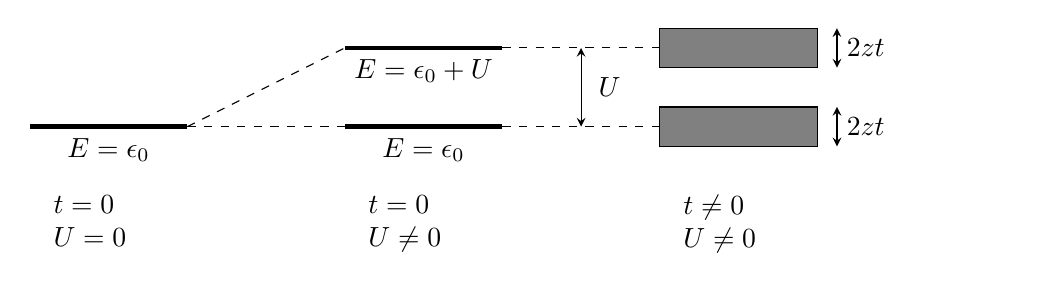
\begin{tikzpicture}
		\draw[level] (0,0) -- node[below] {$ E = \epsilon_0 $} (2,0);
		\draw[connect] (2, 0) -- node{} (4,0);
		\draw[level] (4,0) -- node[below] {$ E = \epsilon_0 $} (6,0);
		\draw[connect] (6, 0) -- node{} (8,0);
		\filldraw [gray, draw = black] (8,-0.25) rectangle (10,0.25);
		\draw[arrow] (10.25, -0.25) -- (10.25, 0.25);
		\node[label, right] at (10.25, 0) {$ 2zt $};
		\draw[connect] (2, 0) -- node{} (4,1);
		\draw[level] (4,1) -- node[below] {$ E = \epsilon_0 + U $} (6,1);
		\draw[connect] (6, 1) -- node{} (8,1);
		\filldraw [gray, draw = black] (8,1-0.25) rectangle (10,1.25);
		\draw[arrow] (10.25, 1-0.25) -- (10.25, 1.25);
		\node[label, right] at (10.25, 1) {$ 2zt $};
		
		\draw[arrow] (7,0) -- (7,1);
		\node[label, right] at (7.1, 0.5) {$ U $};
		
		\node[label, below] at (1.3,-0.75) {$ t = 0 $ \\ $ U=0 $};
		\node[label, below] at (5.3,-0.75) {$ t = 0 $ \\ $ U \ne 0 $};
		\node[label, below] at (9.3,-0.75) {$ t \ne 0 $ \\ $ U \ne 0 $};
	\end{tikzpicture}
	\caption{Degenerate bands split into two in presence of electron-electron interaction, and each band further broadens when electrons are allowed to hop.}\label{fig:splitting}
\end{figure}

It is to be noted here that there is a competition between $ t $ and $ U $. While $ U $ tries to separate the high and low energy states, causing the system to acquire insulator-like nature $ T $ tries to bring them closer, making the system more metallic. At a critical value of $ U_{cr} \approx zt $, the bands start splitting. This is called the Mott-Hubbard transition. The large $ U $ regime causes the formation of distinct Hubbard sub-bands at half-filling and is well within the insulating phase. In this phase, the motion of the electrons now become correlated as electrons try to avoid double occupancy.

In order to treat such systems, we will develop an effective Hamiltonian which filters out the high energy states, leaving us only with the states lying in the lowest Hubbard sub-band.

\section{Classification of hopping events}
We will first separate the Hamiltonian into three parts: parts which do not change the energy of the system by preserving the number of double occupancies, and parts which change the energy by altering the number of double occupancies. In order to filter them, we need to first segregate our basis with respect to the hopping events.

Let us first define a set of local projection operators of the form $ \hat{P}_{i a} = \op{a}_{i} $ which returns an eigenvalue $ 1 $ when the site $ i $ has the occupation $ \ket{a}_i $ as shown in section \ref{sec:spectrum}, otherwise returns 0. Explicitly, the four possible operators are
\begin{align}
	\hat{P}_{j 0} &= \op{0}_j = (1 - \hat{n}_{i, \uparrow})(1 - \hat{n}_{i, \downarrow})\\
	\hat{P}_{j \uparrow} &= \op{\uparrow}_j = \hat{n}_{i, \uparrow} (1 - \hat{n}_{i, \downarrow})\\
	\hat{P}_{j \downarrow} &= \op{\downarrow}_j = \hat{n}_{i, \downarrow} (1 - \hat{n}_{i, \uparrow})\\
	\hat{P}_{j d} &= \op{d}_j = \hat{n}_{i, \uparrow} \hat{n}_{i, \downarrow}
\end{align}
These operators allow us to check whether a state has a given configuration or not.

Consider two sites $ i $ and $ j $ in a system. Suppose, we only want to consider the hopping that starts from a  causes a $ \uparrow $ particle to hop from a singly-occupied $ i $ and make $ j $ doubly occupied after hopping. We can perform these checks with the projectors defined above before and after the hopping and the hopping term now becomes:
\begin{align}
	\hat{P}_{j, d} c^{\dagger}_{j, \uparrow} c_{i, \uparrow} \hat{P}_{i, \uparrow} = \hat{n}_{j, \uparrow}\hat{n}_{j, \downarrow} c^{\dagger}_{j, \uparrow} c_{i, \uparrow} \hat{n}_{i, \uparrow} (1 - \hat{n}_{i, \downarrow}) = \hat{n}_{j, \downarrow} c^{\dagger}_{j, \uparrow} c_{i, \uparrow} (1 - \hat{n}_{i, \downarrow})
\end{align}

This is called a projected hopping, in the sense that this is only a projection of a part of the total space of states that can be created by this hopping.

We see that the above hopping increases the number of doubly occupied sites by one. Collecting all such terms together, we can write the part of the Hamiltonian which increases the number of double occupations in the system by one:

\begin{align}
H^{+}_{t} = -t \sum_{\langle i, j \rangle} \sum_{\sigma} \left[ \hat{n}_{i, -\sigma} c^{\dagger}_{i, \sigma} c_{j, \sigma} (1 - \hat{n}_{j, -\sigma}) + h.c.\right]
\end{align}

\newpage
Similarly, the Hamiltonian for processes which decrease the number of double occupations is given as

\begin{align}
	H^{-}_{t} = -t \sum_{\langle i, j \rangle} \sum_{\sigma} \left[ (1 - \hat{n}_{i, -\sigma}) c^{\dagger}_{i, \sigma} c_{j, \sigma} \hat{n}_{j, -\sigma} + h.c.\right]
\end{align}

There can also be processes which preserve the number of doubly-occupied states, where we check whether both the initial and final states are doubly- \textbf{or} singly-occupied. The Hamiltonian for such processes can be shown to be

\begin{align}
	H^{0}_{t} = -t \sum_{\langle i, j \rangle} \sum_{\sigma} \left[ (1 - \hat{n}_{i, -\sigma}) c^{\dagger}_{i, \sigma} c_{j, \sigma} (1 - \hat{n}_{j, -\sigma}) + \hat{n}_{i, -\sigma} c^{\dagger}_{i, \sigma} c_{j, \sigma} \hat{n}_{j, -\sigma} + h.c.\right]
\end{align}

Combining these three, we can write the band Hamiltonian as

\begin{align}
	H_{\mathrm{band}} = H^{+}_{t} + H^{-}_{t} + H^{0}_{t}
\end{align}

The action of $ H^{\pm}_{t} $ can change the energy of the system and thus, transfers electrons from one sub-band to another. On the other hand, $ H^{0}_{t} $ preserves the energy of a state under its action and thus, restricts an electron to its band. As a result, overall, $ H_{\mathring{band}} $, responsible for the hopping of electrons between sites, leads to a mixing of states between two bands. Also, this results in all hopping not being equally probable, depending on the local environment of the electron. This gives a many-body nature to the kinetic energy part of the Hamiltonian.

\end{document}

